\chapter{Iterative array construction}
\label{chap:unfold}
% Disposition
% * Chapter overview
% * Define our need
% * Tell that there are two possible solutions
% * Present solution one: NDP approach
%   - Show where it breaks down, what are we missing
% * Present solution two: Accelerate approach
%   - Tell how it could be used in Accelerate to solve our problem
%   - That it would be possible to implement directly into the Accelerate architecture
% * Discuss the two approaches
%   - With one world view one is better, with another the other is better.
%   - Depends on the point of view

% (* Tell that we implemented a version in Repa
%   - It did what was necessary for us.
%   - We believe it is an addition that might be worthwhile,
%     as we think it is general enough to suit other problems
%   - Show graph of execution speed versus the best performing
%     solution we have without the new construct)

In this chapter we present our takes on adding support for expressing
iteratively defined arrays. Unfortunately we have not been able to get any of these
extensions completely ready for use and possible inclusion into Nikola.  We
will however give an analysis of what is lacking for a more complete
implementation.

Our need to iteratively define arrays is motivated directly from our case work
on the variants of the recursive Sobol-sequence generator, depicted in
Algorithms \ref{alg:sobol-recursive}, \ref{alg:sobol-parallel-2} and
\ref{alg:lsm-pathgeneration}. While in general the needs for a specific example
does not always warrant language extensions, the case of incremental
construction of output data is arguably a common one, and thus well motivated.

But in isolation, the ability to construct a single array iteratively is
insufficient. It must also be possible to produce multiple iteratively
constructed arrays in parallel. This is due to both the desire for performance and
the desire for expressivity. To meet this end we will analyse two possible ways
to go about this: a nested parallel version and a flat parallel version.

\section{Nested data parallel version}
\label{sec:unfold-mapNest}

Since it is not possible to use recursion in Nikola, we must implement a
primitive iterative operator to incrementally construct arrays.

In Haskell, the function \lstinline{unfoldr} of the
\lstinline{Data.List}-module has the type
\lstinline{(b -> Maybe (a,b)) -> b -> [a]}.

\lstinline{unfoldr f a} recursively populates the element of a list with
\lstinline{f}, as long as it evaluates to a \lstinline{Just}-value. It is a well known
way to construct a list, so we pursue that as an extension.

In Nikola the length of an array is the only intrinsic property shared across
all array representations. Therefore we must know the length of the result array a
priori to evaluating a Nikola \lstinline{unfoldr}.

For a prototype that only uses the last generated element as state, we settle
for the type signature:
\begin{lstlisting}
unfoldr :: (b -> Maybe (a,b)) -> b -> [a]
\end{lstlisting}
It recursively populates the element of a list with \lstinline{f}, as
long as it evaluates to a \lstinline{Just}-value. It is a well known
way to construct a list, which further motivates it as an addition to
Nikola.

In Nikola the length of an array is the only intrinsic property shared
across all array representations. Therefore we must know the length of
the result array a priori to evaluating a Nikola
\lstinline{unfoldr}. For a prototype that only uses the last generated
element as state, we settle for the type signature:
\begin{lstlisting}
unfold :: (Shape sh, IsElem a, Typeable a) 
       => sh -> (sh -> a -> a) -> a -> Array PSH sh a
\end{lstlisting}
In order to be useful however, \lstinline{unfoldr} by itself is not
enough. We need to be able to iteratively produce entire rows or
columns of a matrix as required in Algorithm
\ref{alg:lsm-algorithm}. To remedy this, we set out to explore nested
maps. Again, lacking nested arrays we must use array shapes to express
the structure of our computation.  Like in the case of
\lstinline{unfoldr} we thus must express the resulting shape
beforehand.

The type we eventually arrived at for our maps capable of nesting is depicted
here:
\begin{lstlisting}
mapNest :: (Shape sh, Shape sh', IsElem a, 
            IsElem (Exp t Ix), IsElem b, Source r a)
        => sh'
        -> (Exp t Ix -> Array D sh a -> Array PSH sh' b)
        -> Array r   (sh :. Exp t Ix) a
        -> Array PSH (sh' :. Exp t Ix) b
\end{lstlisting}

While we require the shape \lstinline{sh'} to be specified, there is no guarantee
in the application \lstinline{mapNest f xs} that \lstinline{f x} will not produce an
array exactly the size denoted by \lstinline{sh'}. If the resulting array is
smaller than denoted by \lstinline{sh'}, an eventual manifestation of the map to
memory will leave some cells uninitialized. Similarly, if the resulting array
is not bounded by \lstinline{sh'}, manifesting it will result in writing out of
bounds.

For now we have chosen to accept the existence of these fallacies,
partly because we are concerned with implementing a prototype, and
partly because we do not see any acceptable resolution of the problem
beyond placing the actual array extent rather than just the shape into
the type of the array, as done in \cite{thiemannagda}, but such a
change to Nikola is outside the scope of our project.

Another issue with this definition is the \lstinline{Source r a} restriction on
\lstinline{xs}. If the mapped function does not need to index into the array, it
is an unnecessary restriction to impose.  Similarly, if the mapped function
performs only elementwise operations, preserving the property of being
indexable would be valuable to retain for possible further processing of the
result array.

Risking to further complicate the types, the situation is somewhat remediable
by defining \lstinline{mapNest} as a function in a typeclass parametrised over the
involved array representations, as is already the case for typeclass
\lstinline{Map}.

The most important issue about this definition however, is that it permits
expressing nested array operations, which is not directly executable on the flat
parallel hardware. Treating this issue is the subject of Chapter
\ref{chap:directing-parallelism}.

\subsection{The inadequacies of our implementation}

All our efforts on iterative array construction draw on Nikola's implementation
of 'push' arrays. As mentioned earlier, delayed arrays and push arrays are each
others opposites. Delayed arrays are \lstinline{Source} arrays, and their
manifestation is at the mercy of the consumer of the array. Therefore it is
required that the elements of a delayed array are completely independent from
each other. Push arrays on the other hand are defined as a stream of
index-value pairs, and thus need not obey the same restriction on element
dependence.

Push arrays in Nikola are defined by means of the loop constructor
\lstinline{ForE} of \lstinline{S.Exp}. This loop constructor however, is very
low-level in the sense that it includes as arguments a list of variables to be
looped over and a list of loop bounds corresponding to each of the variables,
and corresponds directly to a \lstinline{for}-loop in C.

% The \lstinline{Shape} typeclass defines an accessible interface for constructing
% for-loops that visit each index of given shape to loop over.  The operation
% \lstinline{seqfor :: Shape sh => sh -> P sh} that we use for constructing our
% loops is defined using the \lstinline{shift} action, and thus needs to be paired
% with an enclosing \lstinline{reset}.  Due to the way that \lstinline{shift} operates,
% what happens is that upon issuing \lstinline{seqfor} in the \lstinline{P} monad, the
% entire surrounding action up to the nearest enclosing reset is placed inside
% the body of the for-loop defined by \lstinline{seqfor}.

However to our regret, using this approach for defining \lstinline{unfold} and
\lstinline{mapNest} proved unfruitful, as the part of the C code generation that
pertains to for-loops in Nikola does not handle cross-iteration data
dependencies properly. It assumes that variables that are overwritten inside
the body of the loop constitute new, fresh variables. Due to our time
constraints we were not able to address this, and have to leave our operations
be for now. If however we disregard this problem, we are not aware of any more
obstacles for implementing our extensions properly.

\section{Flat data parallel version}
Our first attempt at defining an unfolding operation was inspired by the
collective operators of Accelerate.

\begin{lstlisting}
unfold :: (IsElem a, IsElem (Exp t Ix), Shape sh, Source r a)
       => Exp t Ix
       -> (Exp t Ix -> a -> a)
       -> Array r sh a
       -> Array PSH (sh :. Exp t Ix) a
\end{lstlisting}

By avoiding the need for a nested array operations, it is guaranteed
that the resulting unfolded arrays are regular. Furthermore, since the
operation is a mapped version of \lstinline{unfold}, the outer
structure of the computation is completely static, and it is possible
to assign a parallel execution semantics, given that the unfolded
function is executed sequentially.

As such it fits quite well with the other array operations in
Accelerate. If it were to be implemented in Accelerate or Nikola, it
would enable us to express the optimised version of Sobol sequences,
Algorithm \ref{alg:sobol-parallel-2}, which is currently
inexpressible. 

An implementation using the \lstinline{unfold}-operator can be seen in
Algorithm \ref{alg:sobol-unfold}. As $xs$ is a 1D-array, the returned
array, but in memory the values are in the order of the Sobol
sequence. Thus, we just has to tell Nikola or Accelerate to interpret
it differently, which can be done using the built-in
\lstinline{reshape}-function found in both languages.

\begin{algorithm}
  \begin{algorithmic}
    \Function{SobolSkipping-Unfold}{$v$, $n$, $p$, $b$}
    \State $xs \gets$ \textbf{parmap} ($\lambda i$. -> \textsc{SobolInductive}($v$, \textsc{GrayCode} $i$)) $[0..2^{p+b}-1]$
    \State $ys \gets$ \textbf{unfold} $n$ ($\lambda i. \lambda x_i$. \textsc{SkipAhead}($p$, $b$, $i$, $x_i$)) $xs$
    \State \Return $ys$
    \EndFunction
  \end{algorithmic}
  \caption{Parallel Sobol sequence generator. $v$ is the direction
    vector, $n \cdot 2^{p+b}$ is the length of the sequence, $2^p$ is the block size
    and $2^b$ is the number of blocks.}
  \label{alg:sobol-unfold}
\end{algorithm}


\section{Discussion}
Which of the two possible implementations to select depends on ones
point of view. From one point of view, all programs that type checks
should be correct and come with guarantees of good performance. As we
have seen this style does in some cases break program composability,
but the other aspects are certainly also worth pursuing.

In this case, we find that the one invariant a developer has to
manually enforce when applying our \lstinline{mapNest} is worth the
extra cost in man hours, when compared to reading and writing programs
in the style we have seen in Section \todo{ref}.


\section{Repa implementation}
As seen in our survey, we also had problems getting our CPU version to
perform and deliver a speed up, especially Repa did not perform that
well, and only degraded in performance when we added processors.


\begin{figure}
	\centering
\begin{adjustbox}{minipage=1.3\textwidth,margin=0pt \smallskipamount,center}
	\subbottom[Speed-up relative to CUDA implementation.]{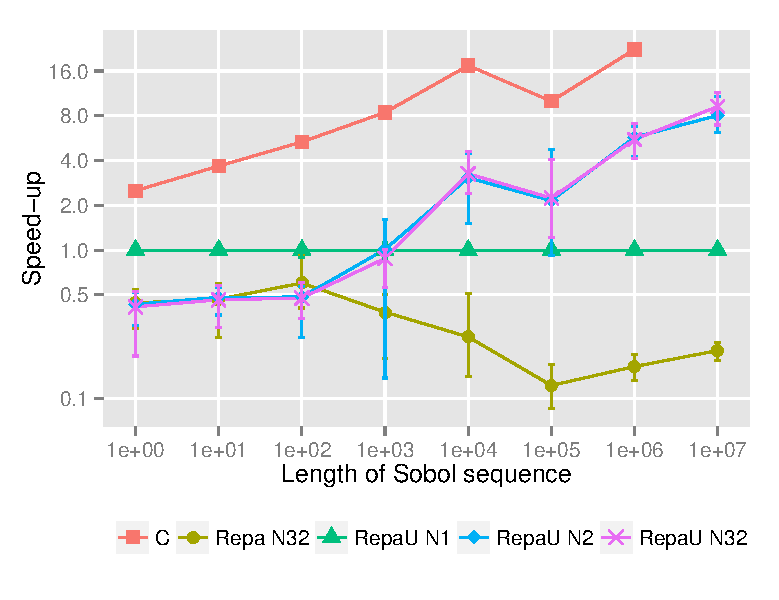
\includegraphics[width=0.5\textwidth]{graphics/final-benchmark/sobol-cpu-RepaUnfold/speedup-graph-final.pdf}\label{fig:sobol-cpu-repaunfold-speedup}}
	\subbottom[Absolute time usage.]{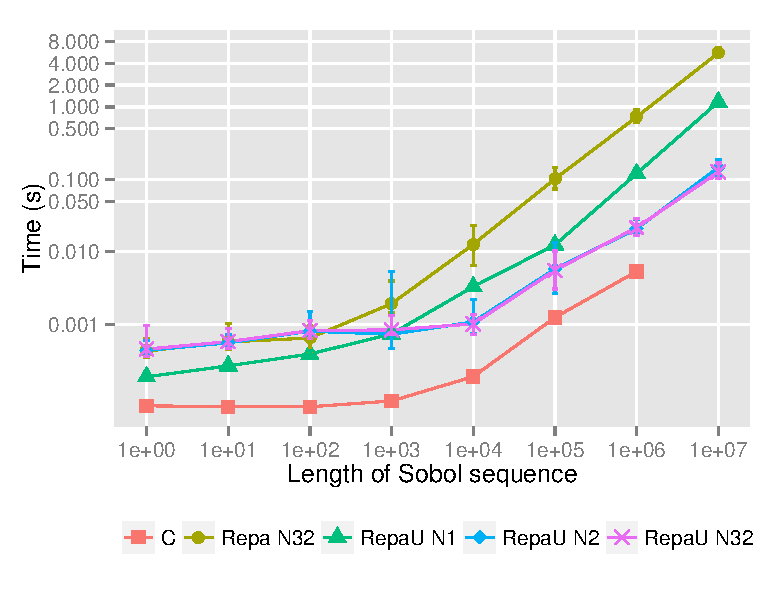
\includegraphics[width=0.5\textwidth]{graphics/final-benchmark/sobol-cpu-RepaUnfold/time-graph-final.pdf}\label{fig:sobol-cpu-repaunfold-time}}
\end{adjustbox}
\caption{Sobol sequence generation on the CPU. We use RepaU to denote
  benchmarks using our new Repa implementation using the
  \lstinline{unfoldChunkedP}-construct.}
\label{fig:sobol-gpu}
\end{figure}


%%% Local Variables:
%%% mode: latex
%%% TeX-master: "../master"
%%% End:
